% !TEX root =  ../MAIN.tex

\section{Data-driven Mutation Analysis: DAMAt}

\renewcommand{\APPR}{DAMAt\xspace{} }

\INDEX{Data-driven mutation analysis} is
a new mutation analysis paradigm
that alters the data exchanged by software components to evaluate the capability of a test suite to detect interoperability faults. 
Data-driven mutation analysis aims to evaluate the effectiveness of a test suite in detecting \INDEX{semantic interoperability \UPDATED{faults}}. 
It is achieved by modifying (i.e., mutating) the data exchanged by CPS components. It generates \INDEX{mutated data} that are representative of data that might be observed at runtime in the presence of a component that behaves differently than expected in the test case; also, it mutates  data that are not automatically corrected by the software 
(e.g., through cyclic redundancy check codes)
%(e.g., through CRC mechanisms, which aim to correct technical interoperability problems) 
and thus causes software failures (i.e., the mutated data shall have a different semantic than the original data). For these reasons, data mutation is driven by a fault model specified by the engineers based on domain knowledge.

Although different types of fault models might be envisioned,
%see background
we propose a technique (\INDEX{data-driven mutation analysis with tables}, \APPR),
which automates data-driven mutation analysis by relying on
a tabular \CHANGED{block model}, itself tailored to the \UPDATED{SUT} through predefined mutation operators.
To concretely perform data mutation at runtime, \APPR relies on a set of \INDEX{mutation probes} that shall be integrated by software engineers into the software layer that handles the communication between components. The runtime behaviour of mutation probes (i.e, what data shall be mutated and how) is driven by the fault model. Thus, \APPR can automatically generate the implementation of mutation probes from the provided fault model.
Depending on the CPS, probes might be inserted either into the \UPDATED{SUT}, into the simulator infrastructure, or both.
For example, Figure~\ref{fig:appr:mutateProbesInserted} shows the architecture of the \ESAIL satellite system with mutation probes integrated into the SVF
%\footnote{Software Validation Facility~\cite{Isasi2019}; it usually includes one or more simulators, an emulator to run the code compiled for the target hardware, and test harnesses.} 
functions that handle communication with external components (PDHU, GPS, and ADCS in this case). 






\APPR works in six steps, which are shown in Figure~\ref{fig:appr:approach}. 
In Step 1, based on the provided methodology and predefined mutation operators, the engineer prepares a fault model specification tailored to the SUT.
% capturing the data format and the types of faults that shall be injected for every data item exchanged by the system components.
In Step 2, \APPR generates a mutation API with the functions that modify the data according to the provided fault model.
In Step 3, the engineer modifies the \UPDATED{SUT} by introducing mutation probes (i.e., invocations to the mutation API) into it.
\REVTOOL{P-2}{Instead of modifying the SUT the engineer may modify the test harness (e.g., the SVF simulator); such choice depends on the software under test, if the test cases are executed through a simulator, such choice prevents introducing damaging changes into the SUT (e.g., delay task execution and break strict real-time requirements).}
In Step 4, \APPR generates and compiles mutants. 
Since the \APPR mutation operators may generate mutated data by applying multiple mutation procedures, \APPR may generate several mutants, one for each \UPDATED{mutation operation (i.e., a mutation procedure configured for a data item, according to our terminology)}.
In Step 5, \APPR executes the test suite with all the mutants including a mutant (i.e., the coverage mutant) which does not  modify the data but traces the coverage of the fault model.
In Step 6, \APPR generates mutation analysis results.

%\UPDATED{
%In our context, the \emph{software under test (SUT)} is the CPS embedded software that is verified by a test suite, which is the target of data-driven mutation analysis. Therefore, we refer to the software developed by the engineers as the \emph{original SUT}. An \emph{SUT mutant} (simply, a \emph{mutant}) is a version of the SUT that integrates a \emph{mutation probe} and shall make test cases fail. 
%%A mutation operator simulates one specific interoperability error (a specific type of that automatically alters data by applying one specific \emph{mutation operation}.
%}



\begin{figure}[h]
	\centering
		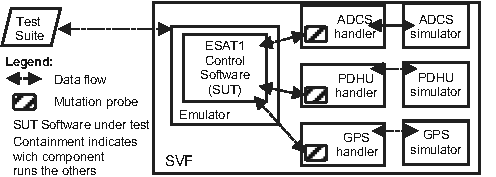
\includegraphics[width=8.4cm]{damat/images/dataMutationExample}
		\caption{\CHANGED{Data mutation probes integrated into \ESAIL.}}
		\label{fig:appr:mutateProbesInserted}
	\end{figure}

\begin{figure}[h]
	\centering
		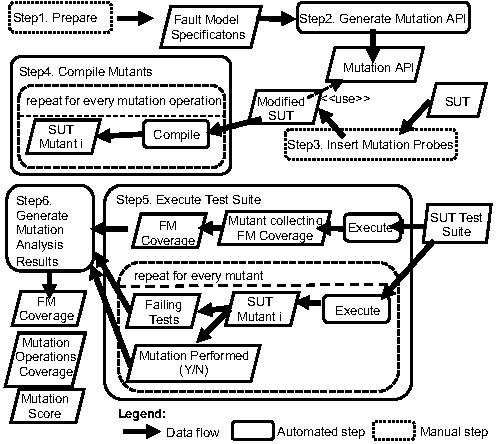
\includegraphics[width=8cm]{damat/images/dataDrivenBufferProcess}
		\caption{The \APPR process.}
		\label{fig:appr:approach}
	\end{figure}


\subsubsection{Fault Model Structure}
\label{sec:faultModelStructure}





The \APPR fault model enables the specification of the format of the data exchanged between components along with the type of faults that may affect such data. 
We refer to the data exchanged by two components as \INDEX{message}; also, each CPS component may generate or receive different \INDEX{message types}.
For a single CPS, more than one fault model can be specified. 

The \APPR fault model enables the modelling of data that is exchanged through a specific data structure: the data buffer. 
The \APPR fault model enables engineers to specify (1) the \emph{position} of each data item in the buffer, (2) their \emph{span}, and (3) their \emph{representation type}. Our current implementation supports six data representation types: int, long int, float, double, bin (i.e., data that should be treated in its binary form), hex (i.e., data that should be treated as hexadecimal).
Further, for each data item, \APPR enables engineers to specify one or more data faults using the mutation operator identifiers. For each operator, the engineer 
shall provide values for the required configuration parameters.
Table~\ref{table:operators} provides the list of mutation operators included in \APPR.

	
	% !TEX root = ../MAIN-DataDrivenMutationAnalysis.tex


\begin{table*}[tb]
\caption{Data-driven mutation operators}
\label{table:operators}
\scriptsize
\begin{tabular}{|p{40mm}|p{90mm}|}
\hline
\textbf{Fault Class}&\textbf{Description}\\
\hline
Value above threshold (VAT)&
Replaces the current value with a value above the threshold T for a delta (\D). 
\\
\hline
Value below threshold (VBT)&
Replaces the current value with a value below the threshold T for a delta (\D). 
\\
\hline
Value out of range (VOR)&
Replaces the current value with a value out of the range $[MIN;MAX]$.\\
\hline
Bit flip (BF)&
A number of bits randomly chosen in the positions between MIN and MAX are flipped.
\\
\hline
Invalid numeric value (INV)&
Replace the current value with a mutated value that is legal (i.e., in the specified range) but different than current value. 
\\
\hline
Illegal Value (IV)
&
Replace the current value with a value that is equal to the parameter \emph{VALUE}. 
\\
\hline
Anomalous Signal Amplitude (ASA)
&
The mutated value is derived by amplifying the observed value by a factor \emph{V} and by adding/removing a constant value \D from it. 
\\
\hline
Signal Shift (SS)
&
The mutated value is derived by adding a value \D to the observed value. 
\\
\hline
Hold Value (HV)
&
This operator keeps repeating an observed value for $V$ times. It emulates a constant signal replacing a signal supposed to vary.
\\
\hline
Fix value above threshold (FVAT)&
In the presence of a value above the threshold, it replaces the current value with a value below the threshold T for a delta \D. 
\\
\hline
Fix value below threshold (FVBT)&
It is the counterpart of FVAT for the operator VBT.
\\
\hline
Fix value out of range (FVOR)&
In the presence of a value out of the range  $[MIN;MAX]$ it replaces the current value with a random value within the range. 
\\
\hline
\end{tabular}
\end{table*}%



Inspired by work on \INDEX{abstract mutation analysis}~\cite{Offutt2006}, we have defined three metrics to evaluate test suites with data-driven mutation analysis: \INDEX{fault model coverage}, \INDEX{mutation operation coverage}, and \INDEX{mutation score}. 
%The first two provide information about the quality of test inputs, whereas the latter provides information about the quality of test oracles \CHANGED{and the test process}. Different from code-driven mutation analysis, data-driven mutation analysis thus enables engineers to distinguish between these two distinct problems affecting test suite effectiveness.
These metrics measure the frequency of the following scenarios: (case 1) the message type targeted by a mutant is never exercised, (case 2) the message type is covered by the test suite but it is not possible to perform some of the mutation operations (e.g., because the test suite does not exercise out-of-range cases), (case 3) the mutation is performed but the test suite does not fail.
\CHANGED{Different from code-driven mutation analysis, these three metrics enable engineers to distinguish between possible test suite shortcomings, including untested message types, uncovered input partitions, poor oracle quality, 
%faulty software, 
and lack of test inputs.}

\INDEX{Fault model coverage (FMC)} is the percentage of fault models covered by the test suite. It provides information about the extent to which the message types actually exchanged by the SUT are exercised and verified by the test suites. 
\CHANGED{Low fault model coverage may indicate that only a small portion of the integrated functionalities have been tested.}

\INDEX{Mutation operation coverage (MOC)} is the percentage of data items that have been mutated at least once, considering only those that belong to the data buffers covered by the test suite. It provides information about the input partitions covered for each data item.
The \INDEX{mutation score (MS)} is the percentage of mutants killed by the test suite \UPDATED{(i.e., leading to at least one test case failure)} among the mutants that target a fault model and for which at least one mutation operation was successfully performed. It provides information about the quality of test oracles; indeed, a mutant that performs a mutation operation and is not killed (i.e., is \emph{live}) indicates that the test suite cannot detect the effect of the mutation (e.g., the presence of warnings in logs).
% or an unexpected output from the system). 
\CHANGED{Also, a low mutation score may indicate missing test input sequences. Indeed, live mutants may be due to either software faults (e.g., the SUT does not provide the correct output for the mutated data item instance) or the software not being in the required state (e.g., input partitions for data items are covered when the software is paused); in such cases, with appropriate input sequences, the  test suite would have discovered the fault or brought the SUT into the required state. Both poor oracles and lack of inputs indicate flaws in the test case definition process (e.g., the stateful nature of the software was ignored).}

